% figures/optionality-mapping.tex
\documentclass[11pt]{article}
\usepackage[margin=1.5cm]{geometry}
\usepackage{tikz}
\usetikzlibrary{arrows.meta}
\pagestyle{empty}
\begin{document}
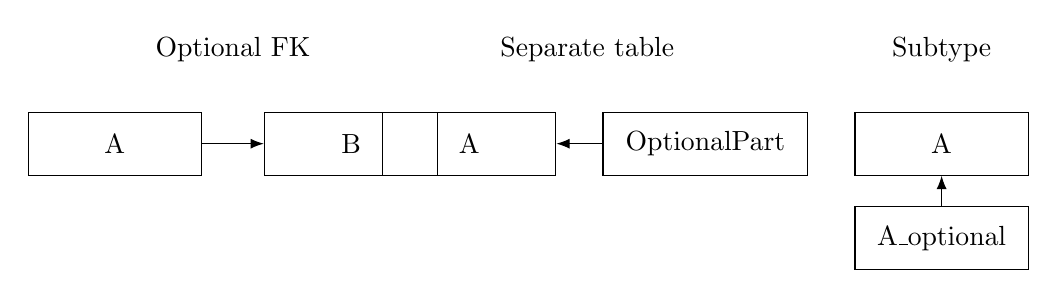
\begin{tikzpicture}[>=Latex]
  % Optional FK
  \node at (-4.5,1.2) {Optional FK};
  \node[draw, rectangle, minimum width=2.2cm, minimum height=0.8cm] (a1) at (-6,0) {A};
  \node[draw, rectangle, minimum width=2.2cm, minimum height=0.8cm] (b1) at (-3,0) {B};
  \draw[->] (a1) -- (b1);

  % Separate table
  \node at (0,1.2) {Separate table};
  \node[draw, rectangle, minimum width=2.2cm, minimum height=0.8cm] (a2) at (-1.5,0) {A};
  \node[draw, rectangle, minimum width=2.6cm, minimum height=0.8cm] (b2) at (1.5,0) {OptionalPart};
  \draw[->] (b2) -- (a2);

  % Subtype
  \node at (4.5,1.2) {Subtype};
  \node[draw, rectangle, minimum width=2.2cm, minimum height=0.8cm] (a3) at (4.5,0) {A};
  \node[draw, rectangle, minimum width=2.2cm, minimum height=0.8cm] (b3) at (4.5,-1.2) {A\_optional};
  \draw[->] (b3) -- (a3);
\end{tikzpicture}
\end{document}
